La scarsità dei risultati ottenuti da BERTopic, ha suscitato alcune perplessità circa l'accuratezza delle informazioni ricavate. Pertanto, è stato sviluppato un ulteriore esperimento volto a identificare le potenziali criticità del modello e a confutare la credibilità dell'ipotesi avanzata al termine della Sezione \ref{4.2.3}: l'assenza di correlazioni tra i documenti e la lista predefinita di topic, potrebbe essere causata dall'impiego da parte dell'algoritmo di una similarità per coseno, inadeguata per operazioni in cui sia necessario catturare sottili differenze semantiche. \vspace{7pt} \\
Il flusso implementativo ricalca gli stessi passaggi illustrati nel paragrafo precedente, a differenza del fatto che il dataset non contiene solamente dati relativi agli articoli del caso di studio, ma si arrichisce di aggiuntive risorse inerenti a pubblicazioni scientifiche in ambito \textbf{quantum computing}. La scelta di combinare contenuti tra loro differenti è motivata dalla volontà di testare la correttezza della tecnica di machine learning, con l'obiettivo di ottenere una netta distinzione al termine dell'elaborazione. \vspace{7pt} \\
Il nuovo dataframe si compone di un totale di $80$ osservazioni, ciascuna completa in ogni feature; le entità aggiuntive sono state recuperate sfruttando la REST API di arXiv, selezionando casualmente $40$ lavori di ricerca in ambito di computazione quantistica.
\begin{lstlisting}[language=python, caption=Creazione e fitting del modello secondo il nuovo dataset]
list_topics = ["Computer Chess", "Quantum Computing"]

model = BERTopic(zeroshot_topic_list=list_topics, zeroshot_min_similarity=.6)
_topics, _ = model.fit_transform(docs, embeddings)
\end{lstlisting}
\begin{lstlisting}[language=python, caption=Recupero e visualizzazione del nuovo dataset finale generato da BERTopic]
df_new_bertopic = model.get_topic_info()
display(df_new_bertopic)
\end{lstlisting}
\begin{figure}[H]
    \centering
    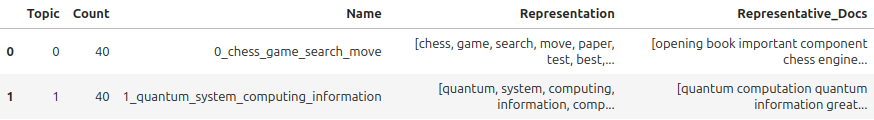
\includegraphics[width=1.0\linewidth]{img/img8.png}
    \label{4.2}
    \caption{Dataset finale generato da BERTopic}
\end{figure}
L'esito finale evidenzia una marcata divisione tra i due gruppi di documenti, valorizzando in questo modo la supposizione iniziale. Il modello BERTopic effettua attività di topic modeling soddisfacenti in casi in cui le informazioni adoperate possano essere contraddistinte in argomenti differenti e non correlati, manifestando quindi minori performance in circostanze in cui le informazioni possano essere ricondotte a molteplici tematiche.